% 修論用の Fig. 1（2026-10-19）: 幅 160 mm、Times（mathptmx）、文字は 8 pt 以上（\footnotesize = 8 pt）、
% 上のタイトルなし。内容は fig1_pipeline_v2.tex と同じ、配置だけ 3 段に。
%   pdflatex -interaction=nonstopmode fig1_pipeline_thesis.tex
\documentclass[10pt,tikz,border=1pt]{standalone}
\usepackage{amsmath,amssymb}\usepackage[T1]{fontenc}\usepackage{mathptmx}\usepackage{bm}
\usetikzlibrary{positioning,arrows.meta,calc}
\definecolor{cCS}{HTML}{0072B2}\definecolor{cCH}{HTML}{009E73}
\definecolor{cDS}{HTML}{E69F00}\definecolor{cDH}{HTML}{D55E00}
\definecolor{ink}{HTML}{222222}\definecolor{mute}{HTML}{6B6B6B}
\definecolor{comp}{HTML}{DCE9F5}\definecolor{viab}{HTML}{F8E3CC}
\begin{document}
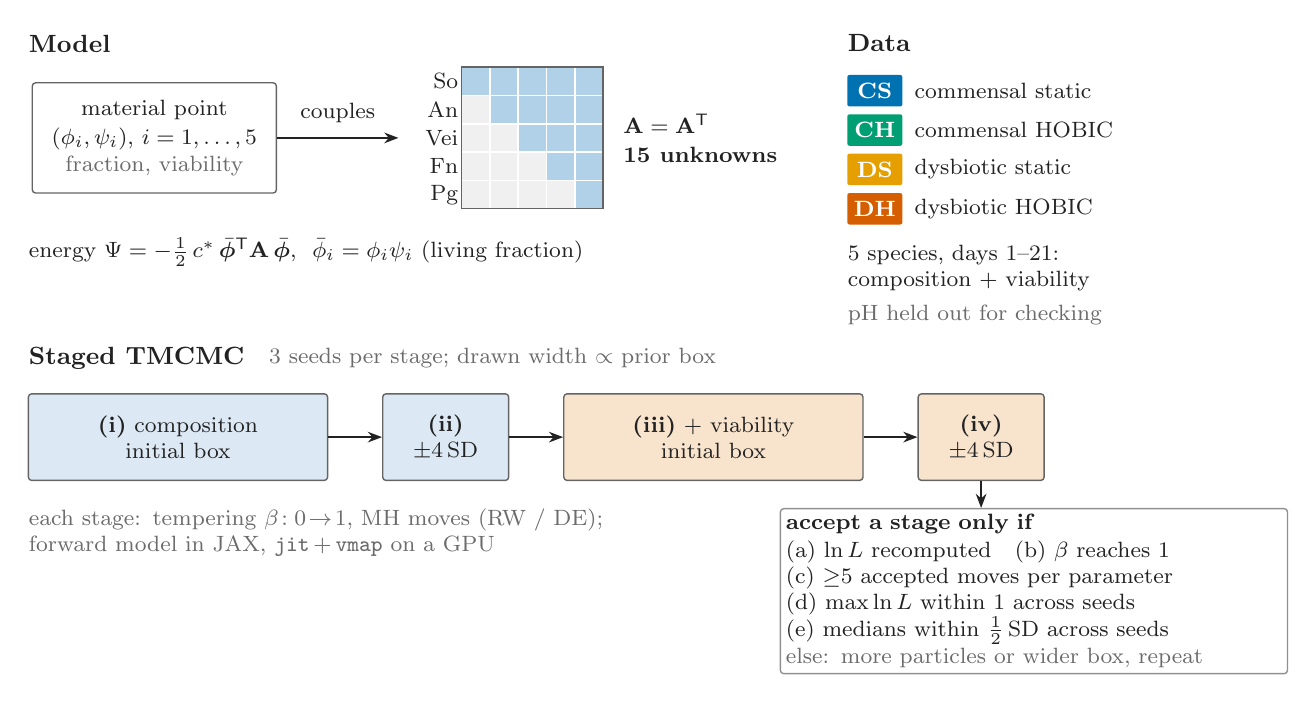
\begin{tikzpicture}[x=1mm,y=1mm,font=\footnotesize,>={Stealth[length=1.8mm]},color=ink,
  head/.style={font=\small\bfseries,anchor=west,inner sep=0pt},
  note/.style={font=\footnotesize,text=mute,inner sep=0pt},
  stage/.style={draw=ink!70,line width=0.5pt,rounded corners=1.2pt,minimum height=11mm,
                align=center,inner sep=1pt,font=\footnotesize},
  chip/.style={rounded corners=0.8pt,minimum width=7mm,minimum height=4mm,inner sep=0pt,
               font=\footnotesize\bfseries,text=white}]
\path (0,-64) rectangle (160,21);

% ---------- Model ----------
\node[head] at (0,19) {Model};
\node[draw=ink!70,line width=0.5pt,rounded corners=1.2pt,align=center,inner sep=2pt,
      minimum width=31mm,minimum height=14mm] (mp) at (16,7)
  {material point\\[1pt] $(\phi_i,\psi_i)$, $i=1,\dots,5$\\[0.5pt]{\color{mute}fraction, viability}};
\def\cs{3.6}
\begin{scope}[shift={(55,-2)}]
  \foreach \i in {0,...,4}{\foreach \j in {0,...,4}{
    \pgfmathtruncatemacro{\up}{\j>=\i ? 1 : 0}
    \ifnum\up=1 \fill[comp!80!cCS] (\j*\cs,{(4-\i)*\cs}) rectangle ++(\cs,\cs);
    \else \fill[black!6] (\j*\cs,{(4-\i)*\cs}) rectangle ++(\cs,\cs); \fi}}
  \draw[white,line width=0.6pt] (0,0) grid[step=\cs] (5*\cs,5*\cs);
  \draw[ink!70,line width=0.5pt] (0,0) rectangle (5*\cs,5*\cs);
  \foreach \s [count=\k from 0] in {So,An,Vei,Fn,Pg}{
    \node[anchor=east,inner sep=1pt] at (0,{(4-\k)*\cs+\cs/2}) {\s};}
  \node[anchor=west,align=left,inner sep=0pt] at (5*\cs+2.5,{2.5*\cs})
    {$\mathbf A=\mathbf A^{\mathsf T}$\\[1pt]\textbf{15 unknowns}};
\end{scope}
\draw[->,line width=0.6pt] (mp.east) -- node[above=0.6mm]{couples} (47,7);
\node[anchor=west,inner sep=0pt] at (0,-7.5)
  {energy $\Psi=-\tfrac12\,c^{*}\,\bar{\bm\phi}^{\mathsf T}\mathbf A\,\bar{\bm\phi}$,\ \ $\bar\phi_i=\phi_i\psi_i$ (living fraction)};

% ---------- Data ----------
\node[head] at (104,19) {Data};
\foreach \t/\c/\l [count=\k from 0] in {CS/cCS/commensal static,CH/cCH/commensal HOBIC,DS/cDS/dysbiotic static,DH/cDH/dysbiotic HOBIC}{
  \node[chip,fill=\c] at (107.5,{13-\k*5}) {\t};
  \node[anchor=west,inner sep=0pt] at (112.5,{13-\k*5}) {\l};}
\node[anchor=west,inner sep=0pt,align=left] at (104,-9.5) {5 species, days 1--21:\\composition $+$ viability};
\node[note,anchor=west] at (104,-15.5) {pH held out for checking};

% ---------- Staged TMCMC ----------
\node[head] (hs) at (0,-21) {Staged TMCMC};
\node[note,anchor=west] at ([xshift=3mm]hs.east) {3 seeds per stage; drawn width $\propto$ prior box};
\def\yb{-31}
\node[stage,fill=comp,minimum width=38mm] (s1) at (19,\yb) {\textbf{(i)} composition\\initial box};
\node[stage,fill=comp,minimum width=16mm] (s2) at (53,\yb) {\textbf{(ii)}\\$\pm4$\,SD};
\node[stage,fill=viab,minimum width=38mm] (s3) at (87,\yb) {\textbf{(iii)} $+$ viability\\initial box};
\node[stage,fill=viab,minimum width=16mm] (s4) at (121,\yb) {\textbf{(iv)}\\$\pm4$\,SD};
\foreach \a/\b in {s1/s2,s2/s3,s3/s4}{\draw[->,line width=0.6pt] (\a.east) -- (\b.west);}
\node[note,anchor=north west,align=left,text width=88mm] at (0,-40)
  {each stage: tempering $\beta\!: 0\!\to\!1$, MH moves (RW / DE);\\
   forward model in JAX, \texttt{jit}\,$+$\,\texttt{vmap} on a GPU};

% ---------- Acceptance ----------
\node[draw=ink!50,line width=0.5pt,rounded corners=1.2pt,anchor=north east,align=left,
      inner sep=2pt,text width=63mm] (acc) at (160,-40) {%
  \textbf{accept a stage only if}\\[0.5pt]
  (a) $\ln L$ recomputed\quad (b) $\beta$ reaches 1\\
  (c) ${\ge}5$ accepted moves per parameter\\
  (d) $\max\ln L$ within 1 across seeds\\
  (e) medians within $\tfrac12$\,SD across seeds\\[0.5pt]
  {\color{mute}else: more particles or wider box, repeat}};
\draw[->,line width=0.6pt] (s4.south) -- (s4.south|-acc.north);
\end{tikzpicture}
\end{document}
